\section{Methodology}\label{sec:methodology}

% \kc{Describe metrics and how to perform  benchmarks here so that in the next section we talk about what specific experiments we are running? Right now they are kind of mixed I think.}

To evaluate the strengths and weaknesses of the LLM-as-a-judge paradigm, we focus on a comparatively controlled setup, in which \judgemodels assess answers of \evaluatormodels on the knowledge benchmark TriviaQA \citep{joshi2017triviaqa}.
With this methodological design, it is possible to focus on the abilities of the judges in isolation, without having to address human disagreement and error at the same time.
In this section, we elaborate the main aspects of our methodology.
\setlength{\parskip}{1pt}
% To obtain a comprehensive picture, we consider several state-of-the-art models often used as judges, a model specifically trained to judge, and several smaller autoregressive models.
% In total, we consider \njudgesword \judgemodels and \nexamtakersword \evaluatormodels.
% More details about the dataset and models are provided in \cref{app:asset-details}.

% \subsection{Benchmark and evaluation metrics}\label{sec:experiments:benchmark}

\paragraph{Evaluation data}
% \subsection{Evaluation data}
%
As our testbed, we use the TriviaQA dataset \citep{joshi2017triviaqa}, consisting of 95K question-answer pairs sourced from 14 trivia and quiz league websites. 
Each question in the train and validation set is annotated with a list of short answers containing a minimal set of facts and evidence documents collected from Wikipedia and the Web.
For our experiments, we use the validation set of the \textit{unfiltered} partition of the benchmark, using the short answers as reference answers.
We use the training set for few-shot examples.

Since experiments require manual annotation of the \evaluatormodel responses, we use a random sample of $400$ questions from the dataset.
In \cref{app:downsamplingstddev}, we show with a bootstrapping test that this sample size has low variance for our main result.
Through experiments described in \cref{subsec:human_alignment}, we establish that humans have high agreement on  judgements of answers given to the questions in the benchmark.

% \subsection{\Evaluatormodels} \label{sec:experiments:evaluationmodel}

\begin{figure*}
    \centering
    \begin{subfigure}[b]{0.415\textwidth}
        \centering
        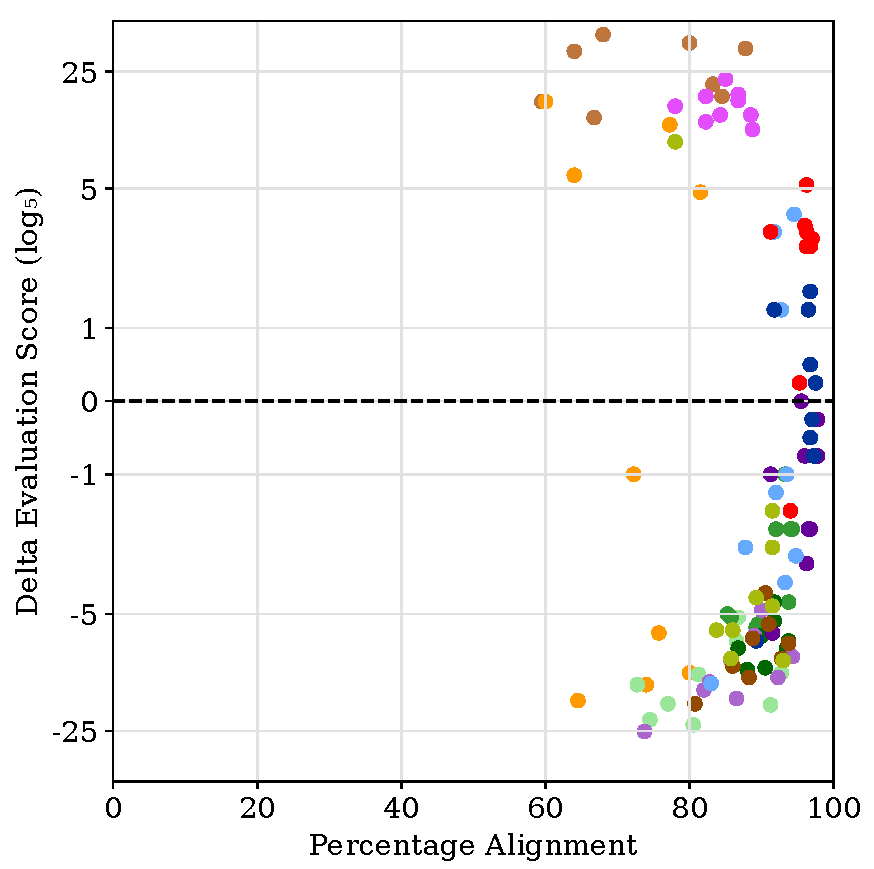
\includegraphics[width=0.9\linewidth]{figures/ScottsPiScoreVariation_aV2.pdf}
        % \vspace{-2mm}
        % \caption{}
        % \vspace{-2mm}
        % \label{fig:pct_aligned_vs_delta}
    \end{subfigure}%
    \begin{subfigure}[b]{0.565\textwidth}
        \centering
        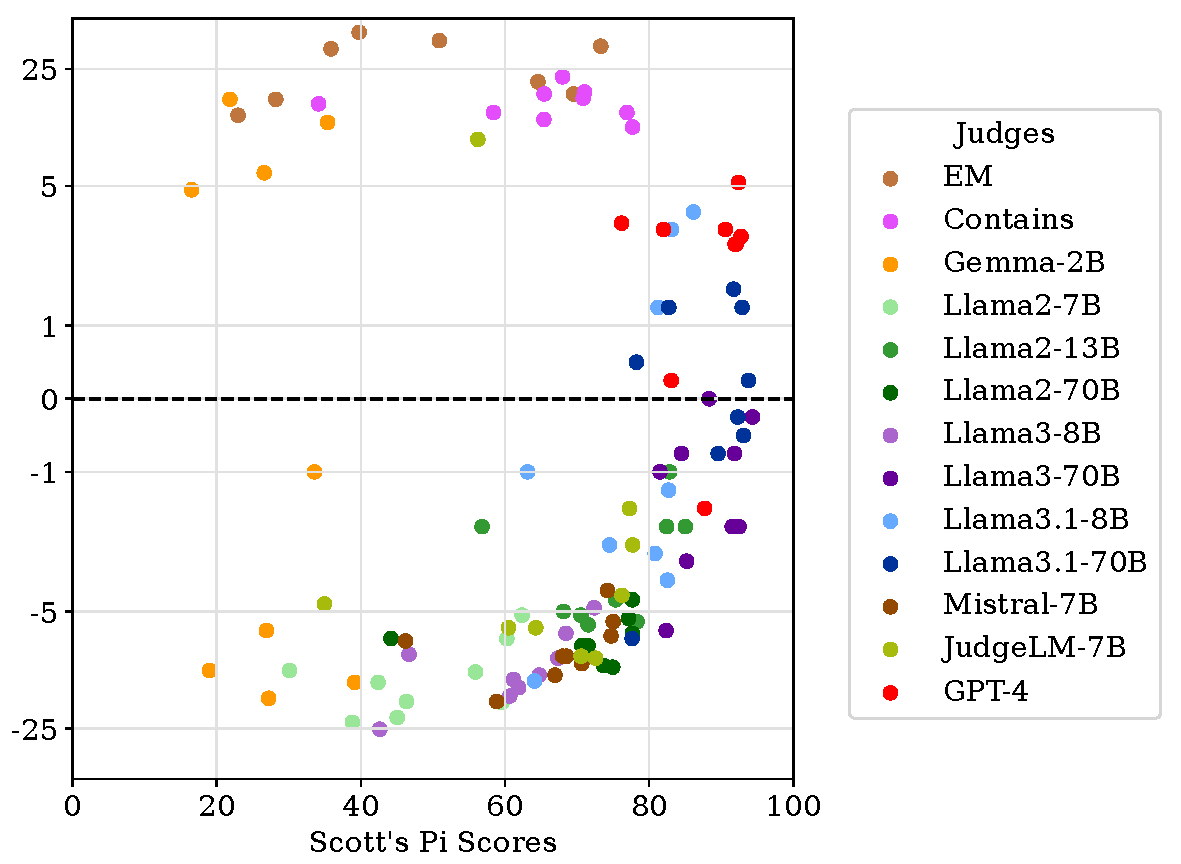
\includegraphics[width=0.9\linewidth]{figures/ScottsPiScoreVariation_bV2.pdf}
        % \vspace{-2mm}
        % \caption{}
        % \vspace{-2mm}
        % \label{fig:pi_vs_delta}
    \end{subfigure}
    \caption{\textbf{Difference with human evaluation scores versus alignment metric.} 
    The delta evaluation score is the difference between the judge and the human score; y-axes are in log scale. 
    Percent alignment (left) shows a very skewwed distribution, making it difficult to distinguish models.
    \scottspi (left) provides a clearer difference between models, and is more indicative of deviation of the gold score.
    % . The left figure shows a skewed distribution for percent agreement and delta evaluation score. Right, we see that highly aligned LLM judges with \scottspi > 0.8 exhibit low variability in scores, while judges with \scottspi < 0.8 demonstrate more variability.
    %impacting their reliability.
    }
    \label{fig:alignment_vs_delta}
\end{figure*}

\paragraph{\Evaluatormodels} \label{subsec:evaluators}
% \subsection{\Evaluatormodels}\label{subsec:evaluators}
%
To understand the strengths and weaknesses of different judges, we consider answers of pre-trained (base) and instruction-tuned (chat) `\evaluatormodels' across a wide variety of model sizes. %, and we examine the quality of the evaluations from different \judgemodels.
In particular, we consider \eval{Llama-2} \citep{touvron2023llama} in 7B, 13B, and 70B parameter sizes for both base and chat versions, \eval{Mistral 7B} \citep{jiang2023mistral} base and chat versions, and \eval{\gpt}\footnote{Accessed via the OpenAI API between Mar 19th, 2024 and Sep 20, 2024.} \citep{achiam2023gpt} as the \evaluatormodels. 
%
The prompts for the \evaluatormodels contain five few-shot examples of (question, answer) pairs from the TriviaQA training set.
The prompts for the instruction-tuned models additionally include a command signaling the model to answer the given question in a succinct manner similar to the provided examples.
The prompts are provided in \cref{app:prompt-templates}.

% \subsection{\Judgemodels} \label{sec:experiments:judgellm}

\paragraph{\Judgemodels}
% \subsection{\Judgemodels}\label{subsec:judges}
%
To get a comprehensive view of the strengths and weaknesses of \judgemodels across different model sizes and architectures, we use instruction-tuned versions of \judge{Llama-2} \citep{touvron2023llama} in 7B, 13B, and 70B sizes, \judge{Llama-3} \citep{meta2024llama3} in 8B and 70B sizes, \judge{Llama-3.1} \citep{dubey2024llama3herdmodels} in 8B and 70B sizes, \judge{Mistral} 7B \citep{jiang2023mistral}, \judge{\gpt} \citep{achiam2023gpt}, \judge{Gemma\;2B} \citep{gemma2024gemma}, and \judge{JudgeLM\;7B} \citep{zhu2023judgelm} as judges. To maintain parity with human and judge evaluation, judge prompts were built from human guidelines in \cref{app:human_annotation_guidelines}. The judges are instructed to respond with only a single word,  \texttt{``correct''} or \texttt{``incorrect''}.
An overview of all \evaluatormodels and \judgemodels is shown in \cref{tab:evaluation}.
For ease of reading, the \judge{\judgemodels} are depicted in a different font than the \eval{\evaluatormodels}.
% \subsection{Evaluation}\label{sec:experiments:baselineandhumanannotation}
% Below, we describe the baselines we compare the \judgemodels with, describe details on how we source human annotations and detail how we compute alignment for the judgemodels.
\paragraph{Baselines} \label{subsec:baselines}
% \subsection{Baselines}\label{subsec:baselines}
As baselines, we use two commonly used lexical evaluation techniques  -- exact match (\judge{EM}) and contains match (\judge{contains}).
For \judge{EM}, a response is considered correct if the response exactly matches one of the reference answers for the given question.
For \judge{contains}, an answer is considered correct if at least one of the reference answers is a sub-string of the response string.
Both EM and contains match are computed in a case-insensitive manner.

% Like exact match evaluation, contains match evaluation is also performed without considering letter casing.
% We compare the judge LLMs assessments with various classical lexical evaluation techniques, such as exact match and contains match, as well as human judgements. In exact match evaluation, if the model's answer exactly matches any of the reference answers for a question, it is evaluated as correct. This evaluation is performed without considering letter casing.
%
% Similarly, contains match evaluation considers an answer correct if the response contains all the words found in any of the reference answers, regardless of their order. Like exact match evaluation, contains match evaluation is also performed without considering letter casing.
%
% The evaluation scores from the judges represent the percentage of questions that the judges deemed correctly answered by the evaluator models, out of the total number of questions in the sample.

\paragraph{Alignment} \label{subsec:alignment}
% \jsubsection{Alignment}\label{subsec:alignment}
We use two metrics to quantify alignment between judges: percent agreement and Scott's Pi coefficient \citep{scott1995scottspi}.%
\footnote{In an earlier version of this paper, we used Cohen's kappa \citep{cohen1960kappa} to measure alignment.
It has since come to our attention that -- despite it's widespread use -- this metric has some well-documented theoretical issues \citep[e.g.][]{pontius2011death,chicco2021matthews}.
For the interested reader, we elaborate on these issues in \cref{app:cohenslimitation}.
}
Percent agreement expresses a simple percentage of the samples on which two annotators agree. 
Scott's Pi, denoted as \scottspi, is an alignment metric that corrects for chance agreement between two annotators and is considered to provide a more robust measure of alignment.
% also takes into account the possibility of chance agreement.
% It is generally considered to provide a more robust measure of alignment. 
Details about the computation of both metrics are given in \cref{app:metrics}.

\begin{figure*}[t]
    \centering
    \begin{subfigure}[b]{0.46\textwidth}
        \centering
        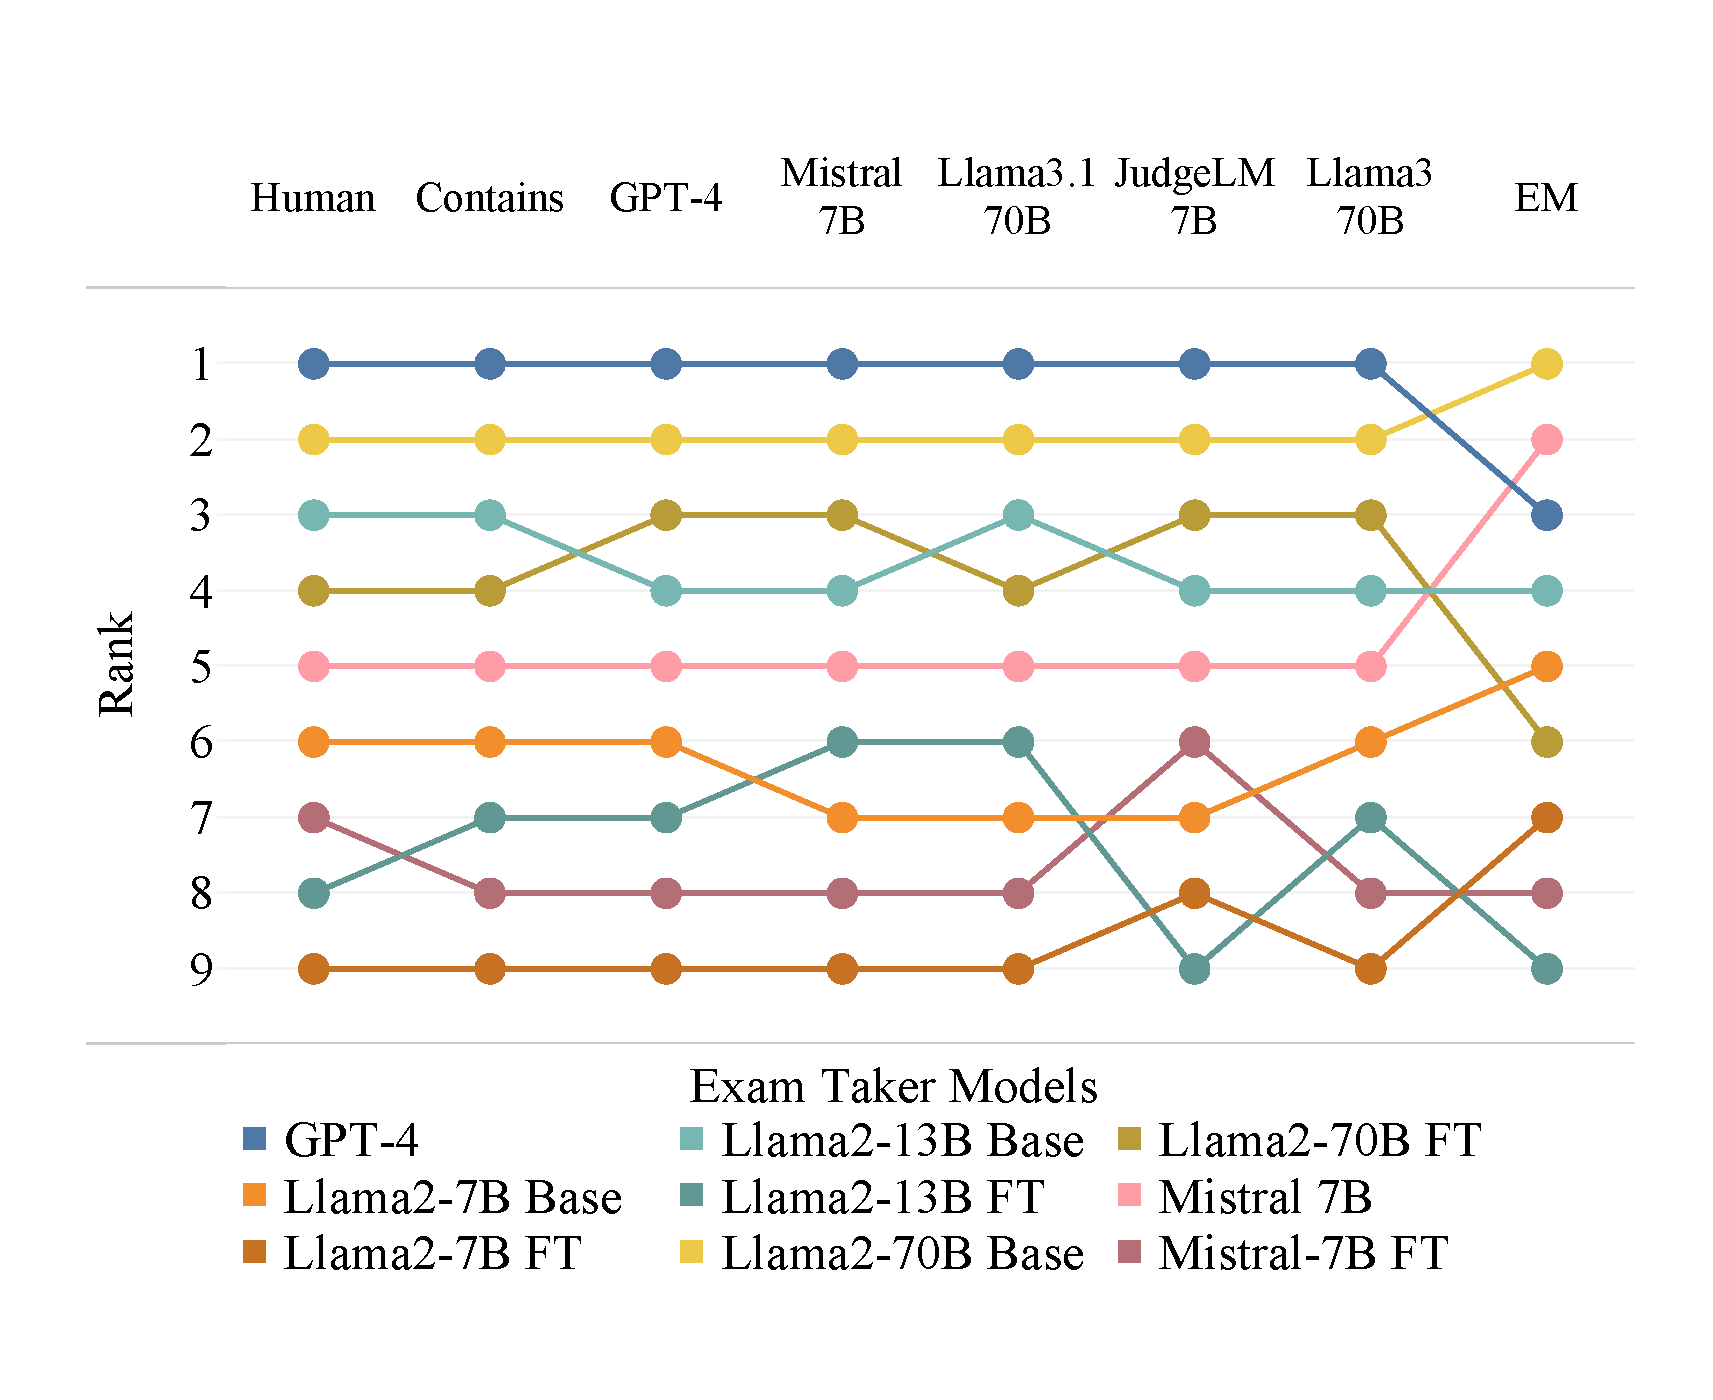
\includegraphics[width=\linewidth]{figures/Rankings_HG.pdf}
        \vspace{-8mm}
        \caption{}
        \vspace{-2mm}
        \label{fig:rankcorrelation}
    \end{subfigure}
    \hfill
    \begin{subfigure}[b]{0.53\textwidth}
        \centering
        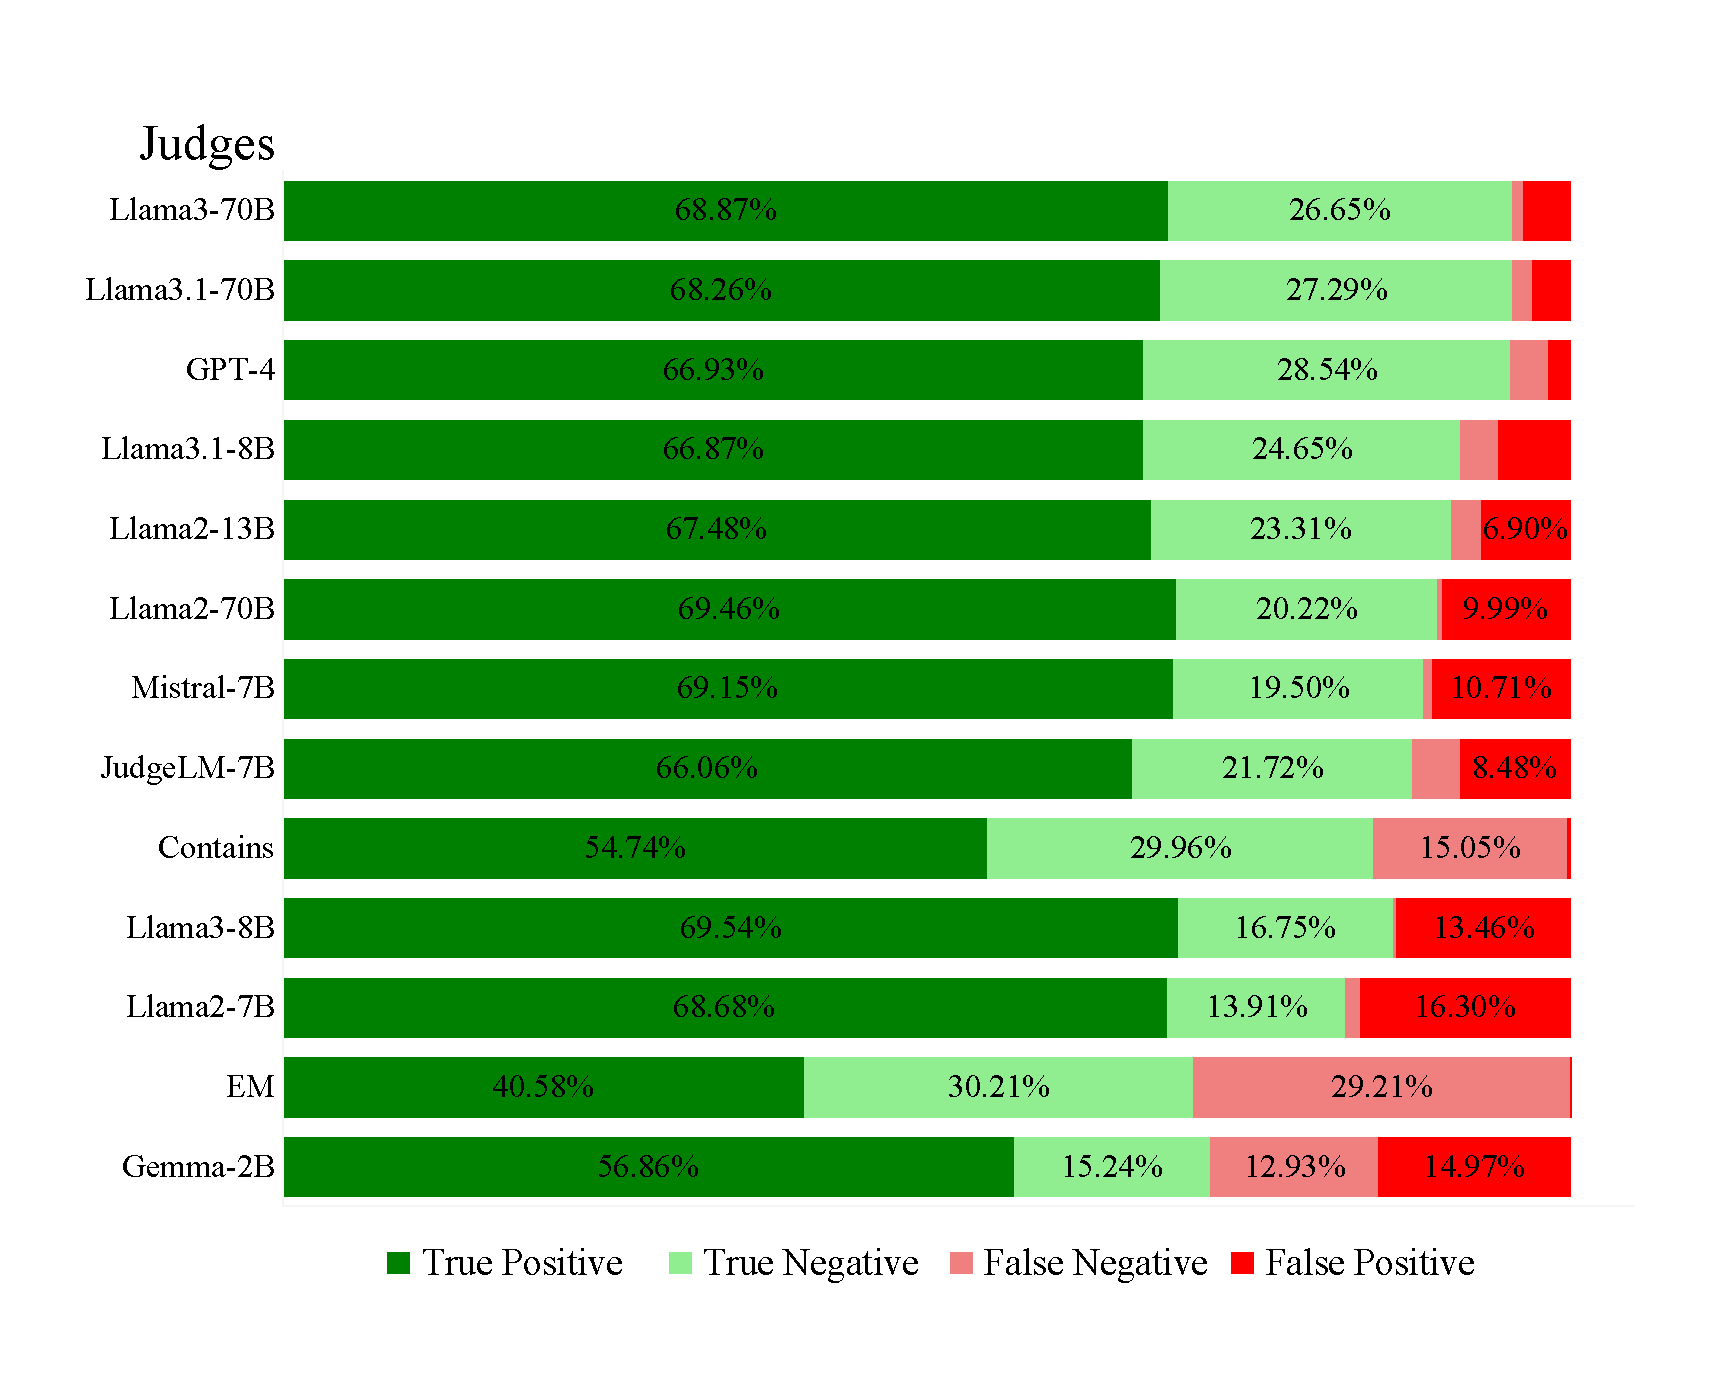
\includegraphics[width=\linewidth, height=5.5cm]{figures/ConfusionMatrixV5.pdf}
        \vspace{-8mm}
        \caption{}
        \vspace{-2mm}
        \label{fig:confusionmatrix}
    \end{subfigure}
    \caption{\textbf{Judge rankings and true/false positives and negatives.} 
    (a) Assigned \evaluatormodel rankings assigned by highly human aligned judges.
    \judge{Contains} stays closely to human-assigned rankings, as well as \judge{\gpt} and \judge{Mistral 7B}. 
    % All judges struggle to distinguish between the poor-performing \evaluatormodels, that may often be closer together.
    (b) False positives and negatives across different \judgemodels, in descending order of human alignment. 
    Both false negatives and false positives increase as human alignment decreases, but well-aligned models tend to produce more false positives than false negatives.
        % \dieuwke{Should increase the font sizes on this one, put the legends on the top and afterwards align appropriately.}
        }\label{fig:ranking_posneg}
\end{figure*}

\paragraph{Human judgements} \label{subsec:human_alignment}
% \subsection{Human judgements}\label{subsec:human_alignment}
As a ground-truth assessment, we obtain human annotations for each \evaluatormodel answer.
The inter-human alignment is calculated between three human judges using the answers to 1200 randomly sampled questions answers; the human guidelines can be found in \cref{app:human_annotation_guidelines}. 
% To compute human inter-annotator agreement, we first conduct an experiment in which three humans judge 600 \eval{Llama-2 7B} \citep{touvron2023llama} answers, randomly sampled from the TriviaQA dataset \citep{joshi2017triviaqa}.
% The human annotators were asked to annotate \evaluatormodel responses that didn't exactly match with one of the references. 
We then determine collective ``Human Judgment'' through a majority vote.
%
% During human annotation, questions marked as correct by the exact match evaluation are skipped, as they are assumed to be annotated correctly by humans. However, these questions are still counted in the final score.

% The average alignment among human evaluators with the majority vote had a \scottspi of $96.2\pm1.07$,%
% \footnote{Coefficient scaled by $100$ for easier comparison with percent alignment.}
% and the average percent agreement was $98.52\%\pm0.42\%$ (pushing the existing SOTA in similar work \citep{zeng2024evaluatinglargelanguagemodels}). 

The average alignment between human evaluators and the majority vote yielded a \scottspi of $96.2\pm1.07$,% 
\footnote{The coefficient is scaled by $100$ for easier comparison with percentage alignment.}
while the average percentage agreement was $98.52\%\pm0.42\%$,  exceeding the alignment previously reported in comparable studies \citep{zeng2024evaluatinglargelanguagemodels}.

The details of this experiment are mentioned in \cref{app:limitations}.
Given this near-perfect alignment score, we consider only one human evaluator per sample for the rest of our experiments, to reduce the overall cost of human annotations. 
The set of questions for which we obtain human annotations is identical for each \evaluatormodel.
%
% After converging on evaluation criteria, we manually annotate 400 questions for each evaluation model.
% Given the high cost of human annotations and near-perfect human alignment between annotators, each evaluation model is annotated by only one human annotator for 400 random sample. 


%\kc{better name?} 
%  We focus on the case of binary annotation, where each evaluation is one of two possible values (e.g., \texttt{correct} or \texttt{incorrect}). 
%  


